\documentclass[11pt,letterpaper]{report}
\usepackage[letterpaper,margin=1in]{geometry}
\usepackage{tikz}

\input{refman.sty}

\def\routine#1{\texttt{#1}\index{#1}}

\title{Base Env: Support routines for parallel programming}
\author{William Gropp}


\begin{document}
\maketitle

\chapter{Introduction}
Base Env is a collection of routines and programs intended to help
with writing and benchmarking parallel programs.
These routines are aimed mostly at MPI programs, but also contain some
routines to work with GPUs.
One goal for these routines is to provide support for node-aware
programming.

\section{Major Elements}
Base Env has two major elements: library routines and applications,
mostly benchmarking programs.

The library routines provide the following capabilities.
\begin{description}
\item[Hardware Configuration]Provide a portable way to access
  information about the hardware configuration, including nodes and
  processor information on a node. This is designed to support
  node-aware programming.
\item[Serializing Code]Provides an efficient way to serialize
  operations, such as printing debugging information.
\item[Unified Memory Management]Provides a simple yet portable way to
  manage memory for both CPUs and GPUs and perform some basic
  initialization and comparisons. Intended primarily to simplify
  benchmark programs.
\item[Benchmarking]Provides routines to help manage timing tests,
  including timing data and controling the tests.
\item[Debugging]Provides integrated support to these routines,
  including easy control through the command line.
\item[Argument Processing]Provides standardized processing of command
  line arguments for these routines.
\item[Utility]Provides miscellaeous utility routines, such as
  collective comparison of values.
\end{description}

Base Env also provides some programs; these are mostly benchmarks but
several provide information about the computing environment.
\begin{description}
\item[hwinfo]Output the hardware configuration, providing details
  including node, socket, NUMA regions, and cores.
\item[ioperf]An I/O benchmark, using MPI I/O.
\item[mpivars]Output the available control and performance variables
  in an MPI implementation.
\item[pingpong]A pingpong performance test, using MPI.
\item[smptest]Benchmark communication performance between two nodes,
  including multiple communicating processes on each node.
\item[stress]A correctness test for interprocess communication, using MPI.
\end{description}
% dttest, mpiexamples

\chapter{Design Overview}
% Overview:
The implementation of Base Env follows a number of standard
practices.
This section summarizes those practices.
Many of these are relevant for understanding the implementation of
Base Env.
The routine naming convention is one exception; that helps to
understand the API provided by Base Env.

\section{Naming Convention}
Most routines in Base Env follow this format:
\begin{verbatim}
   BENV_<package>[<optional-class>]<operation>
\end{verbatim}
In this, \texttt{<package>} is one of the major sections, such as
\texttt{Hwdesc} (for hardware description) or \texttt{Seq} (for
  sequential section).
Some packages might have a subpackage.
One example is \texttt{HwdescNode}, which is focused on information
about the configuration and assignment of processes within a node.

A full list of packages follows:
\begin{description}
\item[Arg]General support for processing command-line arguments
\item[Cart]Provide support for virtual Cartesian process topologies
\item[Darray]Provide support for distributed arrays
\item[Debug]Provide support for debugging the Base Env package
\item[Hwdesc]Provide information about the hardware configuration and
  how processes are assigned to the available hardware
\item[Mem]Support working with memory that may be on an attached
  device, such as a GPU.
\item[Nodecart]An implementation of the MPI Cartesian virtual topology
  routines, taking advantage of the Cart package
\item[Ntest]Estimate the number of times to run a test to ensure the
  test takes enough time relative to the granularity or accuracy of a timer
\item[Seq]Provide for the sequentiql execution of processes in a
  user-defined order
\item[String]Supports working with strings distributed across an MPI
  program, inclusing gather strings of different lengths
\item[TA]Provides a ``timing array'' and support routines for
  analysing timings from benchmarks
\item[Util]
\end{description}

This naming convention is not followed by all routines, though the
routines that don't may be renamed to be consistent with this
convention.
These other routines provide handling of enevironment variables,
specification and printing of integer lists, and similar utility operations.

       Fixme: What to do with the others?
\begin{obeylines}
       CheckSameints
       CreateSubarray
       Get BooleanFromEnv, IntFromEnv, MinMadAvg, NonLocalCounts
       GetSizes, GetSizesArith, GetSizesMult, GetSizesMultDelta
       MeshHaloDatatypes
       PerRankFilename
       PrintInt List, Tuple, NonLocalCounts, RunInfo
       RstringToArray
       ScanScaledInt
\end{obeylines}



\section{Command Line Processing}
Most packages provide routines that offer standard command-line
options.
This ensures that consistent names are used for interfacing with Base
Env packages.
For example, the Hwdesc package provides the routine
\texttt{BENV\_HwdescArg} that processes command-line arguments for that
package.
The routine \texttt{BENV\_HwdescArgPrintUsage} provides a printed
description of those arguments.
These routines allow the user to specify a prefex for every
command-line option to ensure all names are distinct.
For example, for the Hwdesc package, a prefix of \texttt{"-hw"} might
be selected.

\section{Internal Parameters}
Base Env borrows the control variable approach from MPI. Base Env
uses control variables (or \texttt{cvar}s) to control debugging,
default values, and other needs.
These variables typically are named \texttt{cvar\_xxx}.
Command line options are provided to set the values of most control
variables.
These ``cvars'' may also be set through routines defined by different
packages, such as \texttt{BENV\_HwdescCvarSet}.

\section{Error Reporting}
Currently, Base Env tends to write to \texttt{stderr} when an error is
deteched.
This is not optimal, since a package or application that uses Base Env
may want to manage error actions in a different way.
However, internally Base Env has defined some macros to make it easier
to manage error actions, and the longer-term plan is to improve the
flexibility of error actions in Base Env. Contact the author if interested.

\chapter{Hardware Configuration}

These routines, in the \texttt{hwdesc} package, provide information
about the hardware configuration.
To enable debugging of applications or routines that work with the
hardware configuration, various ways are provided to specify the hardware
configuration, including ones that don't match the actual hardware for
the purpose of debugging. This includes using routines, command-line options, or
environment variables.

\section{Representation of the hardware}
There are two different types of information that are needed by a
program that is exploiting the hardware: the \emph{configuration} of
the hardware, i.e., the actual resources (nodes, sockets/chips, NUMA
regions, cores, etc.), and the \emph{assignment} of processes and
threads to that hardware configuration.
Hwdesc attempts to provide a portable implementation of both of these
types of information.

A major challenge with assignment is that the assignment of processes
and threads to the hardware is not necessarily static --- for example,
the operating system may choose to schedule a process or thread on
different cores or even sockets based on factors such as overall load
on the system.
Some operating systems implement \emph{affinity} controls that
constrain the assignment of processes to specific hardware resources.
Base Env currently does not provide access to those controls; you may
find them in packages such as hwloc or as part of the MPI execution
environment.
It is also important to remember that assignment may not be static.
The information provided by Base Env about the assignment of
processes or threads is only guaranteed to be valid at the moment of
the call.
Refer to the documentation for you system about affinities and other
scheduling policies.

Base Env represents the hardware as a hierarchy.
A parallel job is effectively a tree, with the root being all of the
processes in the job on a parallel computer.
Levels in the heirarchy may include nodes, sockets (processor chips),
NUMA regions, and cores.

\begin{figure}
\begin{center}
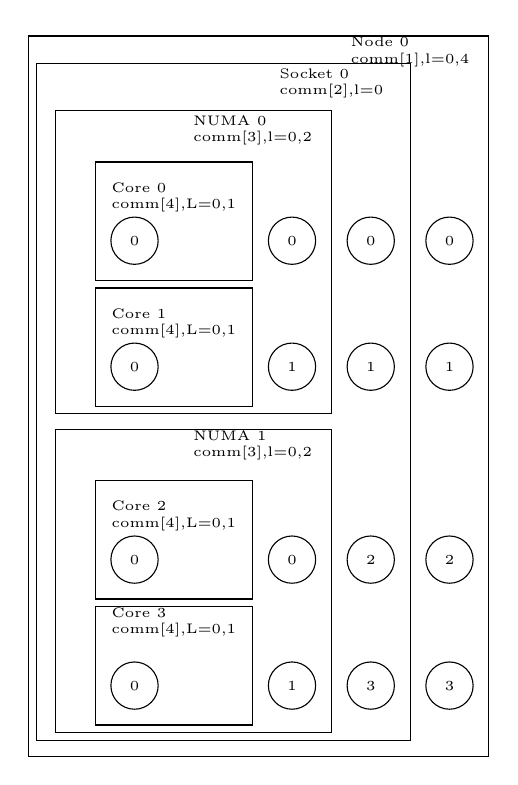
\begin{tikzpicture}[scale=1.0,font=\tiny]
%
% Core 0
\draw[align=left] (0,-1.25cm) rectangle (2cm,-2.75cm)
node at (1cm,-1.7cm) (nodecore0) {Core 0\\comm[4],L=0,1};
\draw (.5cm,-2.25cm) circle (.3cm) node {0};
% Core 1
\draw[align=left] (0,-2.85cm) rectangle (2cm,-4.35cm)
node at (1cm, -3.3cm) (nodecore1) {Core 1\\comm[4],L=0,1};
\draw (.5cm,-3.85cm) circle (.3cm) node {0};
% NUMA 0
\draw[align=left] (-.5cm,-0.6cm) rectangle (3cm,-4.45cm)
node at (2cm,-0.85cm) (numa0) {NUMA 0\\comm[3],l=0,2};
\draw (2.5cm,-2.25cm) circle (.3cm) node {0};
\draw (2.5cm,-3.85cm) circle (.3cm) node {1};

%
% Core 2
\draw[align=left] (0,-5.3cm) rectangle (2cm,-6.8cm)
node at (1cm,-5.75cm) (nodecore0) {Core 2\\comm[4],L=0,1};
\draw (.5cm,-6.3cm) circle (.3cm) node {0};
% Core 3
\draw[align=left] (0,-6.9cm) rectangle (2cm,-8.4cm)
node at (1cm, -7.1cm) (nodecore1) {Core 3\\comm[4],L=0,1};
\draw (.5cm,-7.9cm) circle (.3cm) node {0};
% NUMA 1
\draw[align=left] (-.5cm,-4.65cm) rectangle (3cm,-8.5cm)
node at (2cm,-4.85cm) (numa0) {NUMA 1\\comm[3],l=0,2};
\draw (2.5cm,-6.3cm) circle (.3cm) node {0};
\draw (2.5cm,-7.9cm) circle (.3cm) node {1};

% socket 0
\draw[align=left] (-0.75cm,0cm) rectangle (4cm, -8.6cm)
node at (3cm,-.25cm) (socket0) {Socket 0\\comm[2],l=0};
\draw (3.5cm,-2.25cm) circle (.3cm) node {0};
\draw (3.5cm,-3.85cm) circle (.3cm) node {1};
\draw (3.5cm,-6.3cm) circle (.3cm) node {2};
\draw (3.5cm,-7.9cm) circle (.3cm) node {3};

% Node 0
\draw[align=left] (-0.85cm,.35cm) rectangle (5cm,-8.8cm)
node at (4cm,.15cm) (node0) {Node 0\\comm[1],l=0,4};
\draw (4.5cm,-2.25cm) circle (.3cm) node {0};
\draw (4.5cm,-3.85cm) circle (.3cm) node {1};
\draw (4.5cm,-6.3cm) circle (.3cm) node {2};
\draw (4.5cm,-7.9cm) circle (.3cm) node {3};

(Repeat for node 1)

% Job (0)
\end{tikzpicture}
\end{center}
\caption{}
\label{fig:hwdesc}
\end{figure}

\section{Routines for Hardware Configuration}
Routines in this package are organized in several levels. There are
some high-level routines that are basically drivers that call some of
the lower-level routines

\begin{description}
\item[Command Line Processing]These routines process command line
  arguments for the hardware description routines
 \begin{description}
 \item[BENV\_HwdescArg]Process command line arguments for HW
   description routines
 \item[BENV\_HwdescArgPrintUsage]Print usage information for hwdesc
  command line arguments
 \item[BENV\_HwdescArgConfig]Configure argument names for Hwdesc
 \item[BENV\_HwdescArgCore]Process the core command line arguments for Hwdesc
 \item[BENV\_HwdescArgDebug]Look for debug options for hwdesc routinaes
 \item[BENV\_HwdescArgDebugDecomp]Get arguments for debugging hwdesc usage
 \item[BENV\_HwdescArgPolicy]Get the scheduler policy from argument or
  environment variable
 \end{description}
\item[Parameter Handling]These routines manage hwdescParms
 \begin{description}
 \item[BENV\_HwdescParmInit]Initialize an \texttt{hwdescParms} structure
 \item[BENV\_HwdescParmInitFromEnv]Initialize and hwdescParms from the
  environment
 \item[BENV\_HwdescParmPrint]Print the contents of an hwdesc parms structure
 \item[BENV\_HwdescParmSetFromCvar]Set relevant fields in a parms
  structure from cvars
 \end{description}
\item[Print]These routines print a hardware description in a
  convenient form
 \begin{description}
 \item[BENV\_HwdescPrintAll]Generate a printed description of the
  hwdescCtx description of the system
 \item[BENV\_HwdescPrintLocal]Print the elements of an hwdescCtx
 \item[BENV\_HwdescPrintTuple]Print tuples describing the hardware heirarchy
 \item[BENV\_HwdescToStr]Create a string the describes the hardware hierarchy
 \end{description}
\item[Get Description]Discover hardware configuration and assignment
 \begin{description}
 \item[BENV\_HwdescGetDescGeneral]Create an hwdescCtx using a selected
  method
 \item[Specific Methods]These routines are available through
  BENV\_HwdescGetDescGeneral, but may be appropriate in special cases
  \begin{description}
  \item[BENV\_HwdescGetDescFromDebug]Create an hwdescCtx for debugging
  \item[BENV\_HwdescGetDescFromMPI]Using MPI, get information on the
    HW hierarchy
  \item[BENV\_HwdescGetDescFromPolicy]Create an hwdescCtx from a known
    scheduler policy and known rank in a communicator
  \item[BENV\_HwdescGetDescFromShared]Create a description of the node
    hardware by using infomration on shared memory
  \end{description}
 \item[Node Information]These routines provide information about a node
  \begin{description}
  \item[BENV\_HwdescGetNodeDesc]Update an hwdescCtx with information
    about the node
  \item[BENV\_HwdescNodeGetSockNumaCore]Get information on the socket,
    NUMA region, and core
  \item[BENV\_HwdescNodeGetConfig]Determine the configuration of a node
  \item[BENV\_HwdescNodeGetInfo]Determine the assignent of the calling
    process to hardware elements on a node
  \item[BENV\_HwdescNodeInfoGetcpu]Use getcpu to update hwdesc
    information about the calling process
  \item[BENV\_HwdescNodeInfoPolicy]Use scheduler policy to update hwdesc
    with information about the calling process placement within a node
  \item[BENV\_HwdescNodeInfoSchedgetcpu]Use sched\_getcpu to update
    hwdesc information about the calling process
  \end{description}
 \end{description}
\item[Miscellaneous]These are routines that do not fit into any of the
  above categories
 \begin{description}
 \item[BENV\_HwdescCheckConsistentSizes]
 \item[BENV\_HwdescCreateCtx]
 \item[BENV\_HwdescCvarInit]
 \item[BENV\_HwdescCvarSet]
 \item[BENV\_HwdescFindCommonLevel]
 \item[BENV\_HwdescFindObject]
 \item[BENV\_HwdescFreeCtx]
 \item[BENV\_HwdescGetCoordTuple]
 \item[BENV\_HwdescValidate]
 \end{description}
\end{description}


\section{Example: Determining Node Information for Node-Aware
  Algorithms}
This section describes \file{src/hwinfo.c} at a high level.
Some details are left out; for example, it doesn't discuss
initializing MPI. Please refer to the full code for a
complete, runnable example.


\begin{enumerate}
\item  Create and initialize an HwdescParm structure with information
  to be used in creating a description of the hardware:
\begin{description}
\item[BENV\_HwdescCvarInit]Initialize any control variables (sets defaults)
\item[BENV\_HwdescParmInit]Initialize the HwdescParm
\item[BENV\_HwdescParmUpdateFromEnv]Update from any environment variables
\item[BENV\_HwdescArg]Update from any command line arguments (override
       		      environment variables); this handles the parms and other
		      options.
\item[BENV\_HwdescParSetFromCvar]Update the HwdescParm with values
  from the relevant cvars, including those set through the commandline
\end{description}
\item Create a hardware description, using hwdescParm structure
\begin{description}
\item[BENV\_HwdescGetDescGeneral]Create a hardware description, using one
       of the available methods.
       An alternative is to select a specific approach with routines such as
       BENV\_HwdescGetDescFromShared
\end{description}
\item  Check that the description includes enough node information. If there
       is insufficient information, use a backup method to generate node
       information:
\begin{description}
\item[BENV\_HwdescNodeFindInDesc]Find level in hwdescCtx for node
\item[BENV\_HwdescNodeGetConfig]Get node hardware configuration
\item[BENV\_HwdescNodeGetInfo]Get process assignment to hardware
\item[BENV\_HwdescNodeCombine]Combine node config and info into ??
\item[BENV\_HwdescNodeCombineWithHwdesc]Combine node into existing
       hwdesc
\end{description}
       (Steps 2 and 3 could be combined in a convenience routine)
\item  Optional step: Print the description
       BENV\_HwdescDescPrint
\item  Use the description by accessing the elements of the hwdescCtx
       ?? Need to efine some operations
       	  "partner" on another node
	  Coordinate tuple
\item  Free the description with BENV\_HwdescFreeCtx
\end{enumerate}

\chapter{Benchmarking}
Base Env contains both routines to make it easier to write benchmarks as well
as several benchmarks, especially for communication and I/O performance.

\section{Routines}
There are many challenges in writing benchmarks. Base Env addresses
the several around collecting and analyzing data.
Typically a test might look something like this:
\begin{verbatim}
 t = MPI_Wtime();
for (int i=0; i<ntest; i++) {
    do_thing_to_benchmark();
}
t = (MPI_Wtime()-t)/ntest
\end{verbatim}
This represents a single observation of the time that
\texttt{do\_thing\_to\_benchmark} takes.
A careful benchmark will then run each observation multiple times.

The challenges include:
\begin{enumerate}
\item How many times to run the test (\texttt{ntest} in the above
  loop) --- too few times and
  the test timing will be inaccurate; too many times and the test can
  take too much time.
\item How to store multiple timings for tests, particularly when a
  benchmark is run with different parameters, such as message length.
\item How to analyze the data about the multiple runs, especially for
  parallel program collecting data across multiple processes.
\end{enumerate}

Base Env provides some support for these challenges with the following
packages
\begin{description}
\item[ntest] models the execution time of a test and estimates
  the number of times to run the test to ensure that the measured time
  is long enough
\item[Timearray] provides a way to store and analyze timing data from
  a benchmark program, including ones that measures over a range of
  parameters. It handles parallel programs written using MPI.
\end{description}

\section{Benchmark Programs}

\subsection{smptest}

\subsection{pio}

\subsection{dttest}

\chapter{Serializing Code}
In parallel code, especially when performing output, it is
sometimes necessary to serialize actions - e.g., one process at a
time.
This 

\begin{description}
\item[BENV\_SeqBegin]
\item[BENV\_SeqEnd]
\item[BENV\_SeqChangeOrder]
\end{description}

Here is an example of the use of these routines:
\begin{verbatim}
    MPI_Comm_rank(MPI_COMM_WORLD, &wrank);
    BENV_SeqBegin(MPI_COMM_WORLD);
    printf("This is output from rank %d\n", wrank);
    fflush(stdout);
    BENV_SeqEnd(MPI_COMM_WORLD);
\end{verbatim}
Note that this will not guarantee that the output is seen on stdout in
rank order - that will depend on how the MPI implementation processes
output from different processes.

\chapter{Argument Processing}
Base Env provides standardized argument processing to help applications provide
consistent and complete processing of command line arguments for the components
of Base Env.
Each major Base Env package has a set of routines to process command line
arguments for that package. The routine names are similar, with the
form \texttt{BENV\_<package>Arg<operation>}.
These routines skip unrecognized arguments and update an argument
index for arguments processed.
In addition, most of these routine allow a prefix to be specificed for
the command line arguments, such as \texttt{-hw} for the hwdesc
package, changing arguments such as \texttt{-ncore} to
\texttt{-hw-ncore}.
Finally, most packages provide a way to rename the command line
arguments, using a routine with the name \texttt{BENV\_<package>ArgConfig}.

Need: example of each routine (Config, args, usage, other)

\chapter{Unified Memory Management}
    Overview: Provides a common way to manage memory, on either CPU or GPUs.
    Manage means to allocate and free, as well as to initialize and compare
    to some regular value formulas

Here are the memory types supported:
\begin{description}
\item[MEMOBJ\_MALLOC]Memory allocated with malloc
\item[MEMOBJ\_CUDA]Memory managed with CUDA (NVIDIA)
\item[MEMOBJ\_HIP]Memory managed with HIP (AMD)
\item[MEMOBJ\_SYCL]Memory managed with SYSL (Intel)
\end{description}

Routines (incomplete)
\begin{description}
\item[BENV\_MemDeviceInit]
\item[BENV\_MemAlloc]
\item[BENV\_MemInitValue1D]
\item[BENV\_MemInitValue2D]
\item[BENV\_MemCheckValue1D]
\item[BENV\_MemFree]
\end{description}
Methods that can be invoked on a memory object and data pointers available (incomplete)
\begin{description}
\item[memtodev]
\item[memptr]
\end{description}

Example program that illustrates the use of the memory routines. The full example is in
\file{libsrc/util/tests/memcudatest.c}.
\begin{verbatim}
	BENV_MemDeviceInit(options.mtype);

	mo = BENV_MemAlloc(memlenbytes, options.mtype);

	BENV_MemInitValue1D(mo, memlen, 200, 0, memlen, 0.0, 1.0);

	rc = BENV_MemCheckValue1D(mo, memlen, 200, 0, memlen, 0.0, 1.0);
	/* Make a copy and check locally */
	rc = BENV_MemCheckValue1DWithHost(mo, memlen, 200, 0, memlen, 0.0, 1.0);

	/* Now, update the values on the device, and verify that the checks
	   identify the update */
	for (int j=0; loctest[j] != -3; j++) {
	    value = -100.0;
	    if (loctest[j] > 0)
		offset = loctest[j];
	    else
		offset = memlen + loctest[j];
	    if (offset >= memlen) continue;
	    mo->memtodev((double *)(mo->memptr) + offset, &value, sizeof(double));

	    rc = BENV_MemCheckValue1D(mo, memlen, 200, 0, memlen, 0.0, 1.0);
	    if (rc != offset + 1) {
		fprintf(stderr, "1st error check failed, expected %d, got %d\n",
			offset + 1, rc);
	    }

	    /* Make a copy and check locally */
	    rc = BENV_MemCheckValue1DWithHost(mo, memlen, 200, 0, memlen, 0.0, 1.0);

	    /* Restore old value */
	    value = 200 + offset;
	    mo->memtodev((double *)(mo->memptr) + offset, &value, sizeof(double));
	}

	/* Clean up */
	BENV_MemFree(mo);
    }
\end{verbatim}

\chapter{Debugging Support}
Base Env provides some debugging support, primarily optional printed
output from the routines. These are implemented with a small standard set
of macros and controled through common command-line options.

Common command line options
\begin{description}
\item[-debugclass name{[}:level{]}]Turn on debugging of the named
  class. Optionally, set the level of message. Possible values are
  \texttt{b} for base, \texttt{d} for detail, and \texttt{a} for all.
\item[-debugcalls]Output messages about entering and exiting
  routines. Note that not all functions have implemented this feature.
\item[-debugrank n]Only the process with rank \texttt{n} in
  \texttt{MPI\_COMM\_WORLD} will generate output. By default, all
  processes will output debug information.
\end{description}

Major internal macros:
\begin{description}
\item[CDBGDECL(class)]
\item[CDBGEDECL(class)]
\item[CDBGGDECL(class)]
\item[CDBG(class,level,string)]
\item[CDBGV(class,level,format,...)]
\item[CDBGFCALLENTER]
\item[CDBGFCALLENTERV(format,...)]
\item[CDBGFCALLEXIT]
\end{description}

\chapter{Utility}
Base Env provides a number of utility routines.
These support lists of integers, including determining compressed
representations for regular patterns, printing similar messages over
all processes, string handling, argument processing, and error
messages.

\section{Integer Lists}
routines to process integer lists

\begin{description}
\item[BENV\_PrintIntTuple(fp, n, vals, withEOL)]
\item[BENV\_PrintIntList(fp, n, vals, withEOL)]
\item[BENV\_UtilCompressIntList(n, vec, minrange)]
\item[BENV\_UtilFreeIntList(lst)]
\item[BENV\_UtilIntListToStr(lst)]
\item[BENV\_UtilIntListIsSimple(lst, val, n)]
\item[BENV\_UtilIntListArgDebug(argc, argv, argcnt, prefix)]
\end{description}

\section{Collective Printing}
routines to provide concise printing of statements, particularly for
debugging, across multiple processes.

\section{String Handling}
\begin{description}
\item[BENV\_StringCat2(s1, s2)]
\item[BENV\_StringApp(s1, nstr, ...)]
\end{description}

\section{Argument Processing}
\begin{description}
\item[BENV\_ArgGetint(argnum, argc, argv, val)]
\item[BENV\_ArgGetdouble(argnum, argc, argv, val)]
\item[BENV\_ArgCheckEnoughArgs(argnum, argc, argname, argsneeded,
  printusage)]
\item[BENV\_ARGCHECK(rc,msg,action)](macro)
\end{description}

\section{Error Messages}

\begin{description}
\item[BENV\_ERRMSGV(format,...)](Macro) Writes a message to stderr.
\end{description}

\section{Miscellaneous}

\begin{description}
\item[BENV\_PrintRunInfo(fp,argc,argv)]Print arguments to indicated
  file pointer.
\item[BENV\_GetIntFromEnv(envname, val)]
\item[BENV\_GetBooleanFromEnv(envname, val)]
\item[BENV\_ArrayComputeOffset(nl, coords, sizes, order)]
\end{description}

\chapter{Internal Tests}
Base Env contains many test programs used to test the implementation
of various Base Env routines, both internal and external.

\chapter{Installation}
Base Env uses a configure script to determine available capabilities
and create the makefiles used to build the Base Env libraries.

\begin{verbatim}
   ./configure CC=mpicc FC=mpifort
\end{verbatim}

At the end of the configure run, configure will output a summary of
features, including a table of the hardware configuration and
assignment routines that it tested and it will indicate which ones it
found.
For example, on a Mac laptop, the output includes this near the end:
\begin{verbatim}
configure: Summary of features (with CPP name):
    Compilers:
       C                  mpicc
       Fortran            gfortran
    MPI info:
       SHARED             yes   HAS_MPI_COMM_TYPE_SHARED
       UNGUIDED           yes   HAS_MPI_COMM_TYPE_HW_UNGUIDED
       OMPI Split types   no    HAS_OMPI_HWSPLITTYPES
    Node info:
       getcpu             no    HAVE_GETCPU
       sched_getcpu       no    HAVE_SCHED_GETCPU
       sched_getaffinity  no    HAVE_SCHED_GETAFFINITY
       sysctlbyname       yes   HAVE_SYSCTLBYNAME
       hwloc              no    HAVE_HWLOC
       /proc/cpuinfo      no    HAVE_PROC_CPUINFO

\end{verbatim}


\appendix
\chapter{Example and Test Programs}
\begin{description}
\item[src/hwinfo]
\begin{description}
\item[hwinfo]Use BENV\_HwdescGetDescGeneral to get hardware
	description and BENV\_HwdescPrintAll, BENV\_HwdescPrintCtxLocal,
	and BENV\_HwdescGetCoordTuple to print that description
\item[libsrc/hwdesc/tests]
\begin{description}
\item[gentest]Test the BENV\_HwdescGetDescGeneral routine, using
	command line and/or environment variables to modify the hwdesc
	created
\item[genwnode]Test the BENV\_HwdescGetDescGeneral routine, along
	with the routines to add node information
\item[hwdebug]Test the BENVi\_DistribRankByPolicy routine
\item[hwprint]Test the routines to print a description using
	BENV\_HwdescPrintAll and BENV\_HwdescToStr
	QUERY: Is BENV\_HwdescPrintCtxLocal still defined?
\item[ninfo]Test various routines to determine information about
	the configuration of hardware on nodes and the assignment of
	processes to that hardware, including BENV\_HwdescNodeCombine.
	FIXME: This needs a HwdescNodeArg routine instead of the
	separate tests for things like -nsocket.
\item[nodectest]OLD!!! Tests BENV\_NodeGetNodeComm.
	FIXME: This should be replaced with the appropriate Hwdesc
	routines
\item[ptest]Tests BENV\_HwdescNodeInfoPolicy with
	BENV\_HwdescNodeCombine and BENV\_HwdescNodePrint.
\item[scheddecode]Tests BENVi\_GetNodeSocketFromPolicy
	QUERY: Is this old and deprecated?
\end{description}
\end{description}
\end{description}
	Others include sysctlex, t1, tpolicy

\chapter{Manual Pages}

\input{tex/routines/BENV_ArgCheckEnoughArgs.tex}
\input{tex/routines/BENV_ArgGetdouble.tex}
\input{tex/routines/BENV_ArgGetint.tex}
\input{tex/routines/BENV_ArrayComputeOffset.tex}
\input{tex/routines/BENV_CartDecompCreate.tex}
\input{tex/routines/BENV_CartDecompFree.tex}
\input{tex/routines/BENV_CartDecompGetShift.tex}
\input{tex/routines/BENV_CheckSameInts.tex}
\input{tex/routines/BENV_CreateSubarray.tex}
\input{tex/routines/BENV_DarrayDecomposition.tex}
\input{tex/routines/BENV_DarrayFileType.tex}
\input{tex/routines/BENV_DebugArg.tex}
\input{tex/routines/BENV_DebugArgClass.tex}
\input{tex/routines/BENV_DebugArgCommon.tex}
\input{tex/routines/BENV_DebugArgConfig.tex}
\input{tex/routines/BENV_DebugArgRank.tex}
\input{tex/routines/BENV_DebugFromEnv.tex}
\input{tex/routines/BENV_DebugPostMPIInit.tex}
\input{tex/routines/BENV_GetBooleanFromEnv.tex}
\input{tex/routines/BENV_GetIntFromEnv.tex}
\input{tex/routines/BENV_GetMinMaxAvg.tex}
\input{tex/routines/BENV_GetNonLocalCounts.tex}
\input{tex/routines/BENV_GetSizes.tex}
\input{tex/routines/BENV_GetSizesArith.tex}
\input{tex/routines/BENV_GetSizesMult.tex}
\input{tex/routines/BENV_GetSizesMultDelta.tex}
\input{tex/routines/BENV_HwdescArg.tex}
\input{tex/routines/BENV_HwdescArgConfig.tex}
\input{tex/routines/BENV_HwdescArgCore.tex}
\input{tex/routines/BENV_HwdescArgDebug.tex}
\input{tex/routines/BENV_HwdescArgDebugDecomp.tex}
\input{tex/routines/BENV_HwdescArgPolicy.tex}
\input{tex/routines/BENV_HwdescArgPrintUsage.tex}
\input{tex/routines/BENV_HwdescAssignStr.tex}
\input{tex/routines/BENV_HwdescCheckConsistentSizes.tex}
\input{tex/routines/BENV_HwdescConfigStr.tex}
\input{tex/routines/BENV_HwdescCreateCtx.tex}
\input{tex/routines/BENV_HwdescCvarInit.tex}
\input{tex/routines/BENV_HwdescCvarPrint.tex}
\input{tex/routines/BENV_HwdescCvarSet.tex}
\input{tex/routines/BENV_HwdescFindCommonLevel.tex}
\input{tex/routines/BENV_HwdescFindObject.tex}
\input{tex/routines/BENV_HwdescFreeCtx.tex}
\input{tex/routines/BENV_HwdescGetCoordTuple.tex}
\input{tex/routines/BENV_HwdescGetDescFromDebug.tex}
\input{tex/routines/BENV_HwdescGetDescFromMPI.tex}
\input{tex/routines/BENV_HwdescGetDescFromPolicy.tex}
\input{tex/routines/BENV_HwdescGetDescFromShared.tex}
\input{tex/routines/BENV_HwdescGetDescGeneral.tex}
\input{tex/routines/BENV_HwdescGetNodeDesc.tex}
\input{tex/routines/BENV_HwdescKindStr.tex}
\input{tex/routines/BENV_HwdescNodeConfigCpuinfo.tex}
\input{tex/routines/BENV_HwdescNodeConfigEnv.tex}
\input{tex/routines/BENV_HwdescNodeConfigHwloc.tex}
\input{tex/routines/BENV_HwdescNodeConfigSysctl.tex}
\input{tex/routines/BENV_HwdescNodeGetConfig.tex}
\input{tex/routines/BENV_HwdescNodeGetInfo.tex}
\input{tex/routines/BENV_HwdescNodeGetSockNumaCore.tex}
\input{tex/routines/BENV_HwdescNodeInfoGetcpu.tex}
\input{tex/routines/BENV_HwdescNodeInfoPolicy.tex}
\input{tex/routines/BENV_HwdescNodeInfoSchedgetcpu.tex}
\input{tex/routines/BENV_HwdescNodeNormalize.tex}
\input{tex/routines/BENV_HwdescNodeNormalizeAssign.tex}
\input{tex/routines/BENV_HwdescNodeNormalizeConfig.tex}
\input{tex/routines/BENV_HwdescParmInit.tex}
\input{tex/routines/BENV_HwdescParmPrint.tex}
\input{tex/routines/BENV_HwdescParmSetFromCvar.tex}
\input{tex/routines/BENV_HwdescParmUpdateFromEnv.tex}
\input{tex/routines/BENV_HwdescPrintAll.tex}
\input{tex/routines/BENV_HwdescPrintLocal.tex}
\input{tex/routines/BENV_HwdescPrintTuple.tex}
\input{tex/routines/BENV_HwdescToStr.tex}
\input{tex/routines/BENV_HwdescValidate.tex}
\input{tex/routines/BENV_MemAlloc.tex}
\input{tex/routines/BENV_MemArg.tex}
\input{tex/routines/BENV_MemArgConfig.tex}
\input{tex/routines/BENV_MemArgPrintUsage.tex}
\input{tex/routines/BENV_MemCheckValue.tex}
\input{tex/routines/BENV_MemCheckValue1D.tex}
\input{tex/routines/BENV_MemCheckValue1DWithHost.tex}
\input{tex/routines/BENV_MemCheckValueWithHost.tex}
\input{tex/routines/BENV_MemDebug.tex}
\input{tex/routines/BENV_MemDeviceInit.tex}
\input{tex/routines/BENV_MemFree.tex}
\input{tex/routines/BENV_MemInitValue.tex}
\input{tex/routines/BENV_MemInitValue1D.tex}
\input{tex/routines/BENV_MemInitValue1DWithHost.tex}
\input{tex/routines/BENV_MemInitValueWithHost.tex}
\input{tex/routines/BENV_MeshHaloDatatypes.tex}
\input{tex/routines/BENV_NtestArg.tex}
\input{tex/routines/BENV_NtestArgConfig.tex}
\input{tex/routines/BENV_NtestArgPrintUsage.tex}
\input{tex/routines/BENV_NtestFree.tex}
\input{tex/routines/BENV_NtestGetVal.tex}
\input{tex/routines/BENV_NtestInit.tex}
\input{tex/routines/BENV_NtestInitInfo.tex}
\input{tex/routines/BENV_NtestInitPostMPIInit.tex}
\input{tex/routines/BENV_NtestPrintInfo.tex}
\input{tex/routines/BENV_NtestSaveInfo.tex}
\input{tex/routines/BENV_NtestTimeEst.tex}
\input{tex/routines/BENV_PerRankFilename.tex}
\input{tex/routines/BENV_PrintIntList.tex}
\input{tex/routines/BENV_PrintIntTuple.tex}
\input{tex/routines/BENV_PrintNonLocalCounts.tex}
\input{tex/routines/BENV_PrintRunInfo.tex}
\input{tex/routines/BENV_RstringToArray.tex}
\input{tex/routines/BENV_RstringToArrayOLD.tex}
\input{tex/routines/BENV_ScanScaledInt.tex}
\input{tex/routines/BENV_SeqBegin.tex}
\input{tex/routines/BENV_SeqChangeOrder.tex}
\input{tex/routines/BENV_SeqEnd.tex}
\input{tex/routines/BENV_StringApp.tex}
\input{tex/routines/BENV_StringBcast.tex}
\input{tex/routines/BENV_StringCat2.tex}
\input{tex/routines/BENV_StringCheckSame.tex}
\input{tex/routines/BENV_StringConcatFree.tex}
\input{tex/routines/BENV_StringRecv.tex}
\input{tex/routines/BENV_StringSend.tex}
\input{tex/routines/BENV_TAFindQuartiles.tex}
\input{tex/routines/BENV_TAFree.tex}
\input{tex/routines/BENV_TAInit.tex}
\input{tex/routines/BENV_TAPlotCandlestickData.tex}
\input{tex/routines/BENV_TAPrintCandlestickData.tex}
\input{tex/routines/BENV_TASetVal3.tex}
\input{tex/routines/BENV_UtilAppendIntArray.tex}
\input{tex/routines/BENV_UtilCompressIntList.tex}
\input{tex/routines/BENV_UtilCreateIntArray.tex}
\input{tex/routines/BENV_UtilFreeIntArray.tex}
\input{tex/routines/BENV_UtilFreeIntList.tex}
\input{tex/routines/BENV_UtilIntArrayToIntList.tex}
\input{tex/routines/BENV_UtilIntListArgDebug.tex}
\input{tex/routines/BENV_UtilIntListIsSimple.tex}
\input{tex/routines/BENV_UtilIntListToStr.tex}
\input{tex/routines/MPIX_Comm_split_method.tex}
\input{tex/routines/MPIX_Comm_split_unguided.tex}
\input{tex/routines/MPIX_Nodecart_coords.tex}
\input{tex/routines/MPIX_Nodecart_create_from_hierarchy_local.tex}
\input{tex/routines/MPIX_Nodecart_create_from_hierarchy.tex}
\input{tex/routines/MPIX_Nodecart_create.tex}
\input{tex/routines/MPIX_Nodecart_cvar_set.tex}
\input{tex/routines/MPIX_Nodecart_get.tex}
\input{tex/routines/MPIX_Nodecart_rank.tex}
\input{tex/routines/MPIX_Nodecart_shift.tex}
\input{tex/routines/MPIX_Nodecart_sub.tex}
\input{tex/routines/MPIX_Nodecartdim_get.tex}

% Add index only when \routine is used and we add index processing to
% the build process for this document
%\chapter{Index}

\end{document}
